%% LyX 1.6.0 created this file.  For more info, see http://www.lyx.org/.
%% Do not edit unless you really know what you are doing.
\documentclass[english]{beamer}
\usepackage{mathptmx}
\usepackage[T1]{fontenc}
\usepackage[latin9]{inputenc}
\usepackage{amsmath}
\usepackage{amssymb}

\makeatletter
%%%%%%%%%%%%%%%%%%%%%%%%%%%%%% Textclass specific LaTeX commands.
 % this default might be overridden by plain title style
 \newcommand\makebeamertitle{\frame{\maketitle}}%
 \AtBeginDocument{
   \let\origtableofcontents=\tableofcontents
   \def\tableofcontents{\@ifnextchar[{\origtableofcontents}{\gobbletableofcontents}}
   \def\gobbletableofcontents#1{\origtableofcontents}
 }
 \makeatletter
 \long\def\lyxframe#1{\@lyxframe#1\@lyxframestop}%
 \def\@lyxframe{\@ifnextchar<{\@@lyxframe}{\@@lyxframe<*>}}%
 \def\@@lyxframe<#1>{\@ifnextchar[{\@@@lyxframe<#1>}{\@@@lyxframe<#1>[]}}
 \def\@@@lyxframe<#1>[{\@ifnextchar<{\@@@@@lyxframe<#1>[}{\@@@@lyxframe<#1>[<*>][}}
 \def\@@@@@lyxframe<#1>[#2]{\@ifnextchar[{\@@@@lyxframe<#1>[#2]}{\@@@@lyxframe<#1>[#2][]}}
 \long\def\@@@@lyxframe<#1>[#2][#3]#4\@lyxframestop#5\lyxframeend{%
   \frame<#1>[#2][#3]{\frametitle{#4}#5}}
 \makeatother
 \def\lyxframeend{} % In case there is a superfluous frame end

%%%%%%%%%%%%%%%%%%%%%%%%%%%%%% User specified LaTeX commands.
\usetheme{Warsaw}
% or ...

\setbeamercovered{transparent}
% or whatever (possibly just delete it)

\makeatother

\usepackage{babel}

\begin{document}

\title{Elliptic Curve Cryptography}


\author{G. Aleksandrowicz\inst{1} \and B. Hess\inst{2}}


\institute{\inst{1}Department of Computer Science, Technion \and \inst{2} Department of Computer Science, ETH Zurich}


%\date{Technion - Israel Institute of Technology\and \inst{2}Department
%of Theoretical Philosophy}


%\date{University of Else}


\date{Project in Computer Security, 2009}

\makebeamertitle

\lyxframeend{}

\lyxframe{Outline}

\tableofcontents{}

\lyxframeend{}

\section{Elliptic Curves}
\lyxframe{Definition}
\begin{itemize}
\item An Elliptic Curve is the set of solutions of an equation of the form
$y^{2}=x^{3}+ax+b$ over some field $\mathbb{F}$.
\item Usually denoted $E_{\mathbb{F}}$.
\item There is a small condition on $a,b$ ($4a^{3}+27b^{2}\ne0$)
\item If $\mbox{char}\mathbb{F}=2,3$ the equation is a little more complex...
\item We also consider a solution {}``at infinity'', $O$.
\end{itemize}
\lyxframeend{}

\lyxframe{The Group Operation - Illustration}
\begin{figure}[h]
\centering
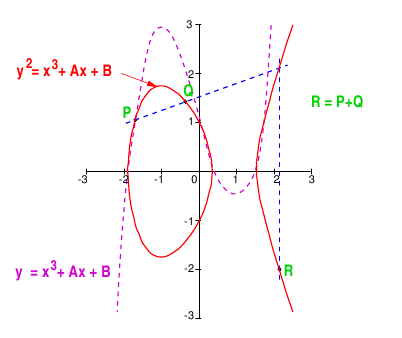
\includegraphics[scale=0.4]{ecaddition.png}
\caption{Addition of two points $P+Q$ in an EC}
\label{tradebefore}
\end{figure}
\lyxframeend{}

\lyxframe{Enter Elliptic Curves}
\begin{itemize}
\item Elliptic Curves provide a wide variety of groups, similar to $\mathbb{Z}_{n}^{*}$
but more complex.
\item Diffie-Hellman and El-Gamal can be reproduced in this setting.
\item The discrete logarithm problem is much harder - i.e. the index calculus
method is not applicable.
\item This results in much smaller key sizes (100-200 bits).
\item The problem: More costly to generate, more costly to operate.
\end{itemize}

\lyxframeend{}

\lyxframe{Encoding Text to an Elliptic Curve}
\begin{itemize}
 \item Our implementation encodes ASCII text to points on the EC.
 \begin{itemize}
  \item This is no restriction. Arbitrary files can be encoded to ASCII (e.g. with base64)
 \end{itemize}
 \item The encoding works the following way ($k$ is the maximum point size in bytes):
 \begin{itemize}
  \item $k-1$ characters are appended bytewise to the x-coordinate.
  \item 1 random byte is appended $\rightarrow$ padding.
  \item The corresponding y-coordinate is computed.
  \item If no y-coordinate exists, another random padding is selected.
 \end{itemize}
 \item Half of the x-coordinates correspond to a valid point.
 \item Padding serves two purposes:
 \begin{itemize}
  \item Finding a valid point
  \item Introducing non-determinism.
 \end{itemize}
\end{itemize}
\lyxframeend{}

\lyxframe{ECC ElGamal Results}
\begin{figure}[h]
\centering
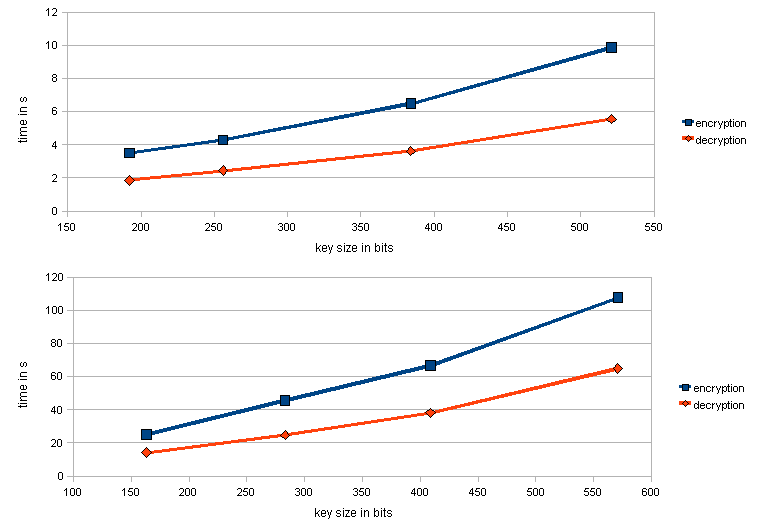
\includegraphics[scale=0.33]{dia2.png}
\caption{3.3KB file, top: prime curves, bottom: binary curves}
\label{agm1}
\end{figure}
\lyxframeend{}

\lyxframe{ECC ElGamal Evaluation}
\begin{itemize}
 \item Timings are not very competitive, there is much potential for optimizations.
 \item Binary version uses binary field arithmetic, built from scratch.
 \begin{itemize}
  \item Using specialized libraries would improve the performance.
  \item Optimizations for reduction trinomials could be added.
 \end{itemize}

\end{itemize}

\lyxframeend{}

\lyxframe{Point Counting with AGM (1)}
\begin{itemize}
\item The \emph{Arithmetic-Geometric Mean} is defined as the sequence:\end{itemize}
\begin{fact}%{}
$a_0=a$, $b_0=b$, $a_{n+1}=\frac{1}{2}(a_n+b_n)$, $b_{n+1}=\sqrt{a_nb_n}$\end{fact}%{}
\begin{itemize}
\item Gauss discovered: for $n\rightarrow\infty$, $a$ and $b$ will converge:\end{itemize}
\begin{fact}%{}
$AGM(a,b):=\lim\limits_{n \rightarrow \infty}{a_n}=\lim\limits_{n \rightarrow \infty}{b_n}$\end{fact}%{}
\begin{itemize}
\item Classical application of AGM: approximation of number $\pi$.
\end{itemize}

\lyxframeend{}

\lyxframe{Point Counting with AGM (2)}
\begin{itemize}
\item Mestre (2000) applied AGM for point counting in elliptic curves over $\mathbb{F}_{2^d}$, EC: $y^2+xy=x^3+c$
\item The EC order is determined by its \emph{trace} $t$: $|EC|=2^d+1-t$
\item $t$ is computed using AGM:
\end{itemize}
\begin{fact}$a=1$, $b=1+8c$, $t=\frac{a_0}{AGM(a,b)}=\frac{a_0}{a_d}$\end{fact}%{}
\begin{itemize}
\item Difficulty: $a$ and $b$ are so-called \emph{2-adic polynomials}
\item These are polynomials of degree $d$, with coefficients modulus $2^N$. $N$ is called the \emph{precision}.
\end{itemize}
\lyxframeend{}

\lyxframe{AGM implementation}
\begin{itemize}
\item Current programming libraries don't implement 2-adic arithmetic.
\item Our 2-adic implementation includes: addition/subtraction, multiplication, modular reduction, division, square root, inverse polynomial.
\item Polynomial multiplication is the major bottleneck. It can be highly optimized using FFT.
\item Comparison between AGM with ``naive'' multiplication and optimized variant from \emph{NTL} shows enormeous performance improvements:
\begin{itemize}
\item AGM on a 283 bit EC. Naive version: 30 minutes. Optimized version: 1.5 seconds.
\end{itemize}
\end{itemize}
\lyxframeend{}

\lyxframe{AGM Point Counting Evaluation}
\begin{figure}[h]
\centering
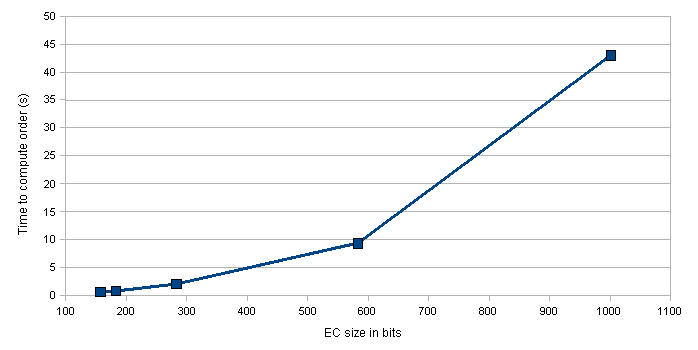
\includegraphics[scale=0.35]{dia1.png}
\caption{AGM times with variable EC sizes, 1.8GHz Core Duo}
\label{agm1}
\end{figure}
\lyxframeend{}

\lyxframe{AGM - Further Work}
\begin{itemize}
\item Not all random curves are secure. Curve order should exceed a certain value.
\begin{itemize}
\item Use a ``early abort'' strategy to quickly skip insecure curves.
\end{itemize}
\item Even faster libraries for polyomial multiplication exist today
\begin{itemize}
 \item Use ``FLINT'' instead of NTL.
\end{itemize}
\item Other point counting methods exist, with lower asymptoic complexity.
\begin{itemize}
 \item AGM has $O(n^{3+\epsilon})$ complexity.
 \item Newer method has $O(n^{2+\epsilon})$ complexity.
 \item Practical comparison would be interesting.
\end{itemize}
\item Comparison with binary field CM.
\end{itemize}
\lyxframeend{}


\appendix

\section*{Appendix}


\lyxframeend{}\subsection*{For Further Reading}


\lyxframeend{}\lyxframe{[allowframebreaks]For Further Reading}

\beamertemplatebookbibitems
\begin{thebibliography}{1}
\bibitem{HMV}D. Hankerson, A. Menezes, S. Vanstone. Guide to Elliptic
Curve Cryptography. Springer, 2004.
\bibitem{HMV}H. Baier, J. Buchmann. Generation Methods of Elliptic Curves. 2002.	\beamertemplatearticlebibitems

\end{thebibliography}

\lyxframeend{}
\end{document}
